\documentclass[pdf,aspectratio=169]{beamer}
\usepackage[]{hyperref,graphicx,siunitx,booktabs,lmodern}
\usepackage{physics}
\usepackage{em-commands}
\mode<presentation>{\usetheme{EM}}

%Question Numbering
\newcounter{questionnumber}
\newcommand{\qnum}{%
	\stepcounter{questionnumber}%
	Q\arabic{questionnumber}
}
\resetcounteronoverlays{questionnumber}

\graphicspath{ {../Images/} }

\sisetup{per-mode=symbol}

\tikzstyle{plate}=[draw, very thick, minimum width=4cm, minimum height=1cm, fill=gray!40, anchor=south]

%preamble
\title{Time to Meditate}
\date{November 28, 2018}
\author{Jed Rembold}

\begin{document}
\renewcommand{\theenumi}{\Alph{enumi}}

\begin{frame}{Announcements}
	\begin{itemize}
		\item Homework
			\begin{itemize}
				\item Homework 11 due tonight!
				\item I'm aiming to get HW12 (the last one!) out by this evening
			\end{itemize}
		\item I'm handing back the take-home portions (or you already got an email from me)
		\item I'm working on getting a new grade report out so you can have a good idea where you stand going into the last stretch.
		\item Finish reading 7.1 and read 7.2.1 by Friday
	\end{itemize}
\end{frame}

\begin{frame}{\qnum}
	What are the units for the area under a $\af$-$\mf$ hysteresis curve?
	\begin{enumerate}
		\item $\displaystyle\si[per-mode=fraction]{\square\tesla \ampere\per\newton}$
		\item \alert<2>{$\displaystyle\si[per-mode=fraction]{\newton\per\square\meter}$}
		\item $\displaystyle\si[per-mode=fraction]{\square\tesla}$
		\item $\displaystyle\si[per-mode=fraction]{\tesla\ampere\per\square\newton}$
	\end{enumerate}
\end{frame}

\begin{frame}{\qnum}
	\begin{columns}
		\column{0.5\textwidth}
		A thin electric current $\mcur$ flows along a copper wire (low resistivity) into a thick resistor made of carbon (high resistivity), then back into another copper wire. In which material is the electric field the largest?
		\begin{enumerate}
			\item In the copper wire
			\item In the carbon resistor
			\item It is the same in both copper and carbon
			\item \alert<2>{It depends on the exact sizes of copper wire and carbon resistor}
		\end{enumerate}
		
		\column{0.5\textwidth}
		\begin{center}
			\begin{tikzpicture}
				\pic (r) at (0,0) {cyl=red/1/3/3};
				\path[very thick] 
					(0,0) edge +(0,2)
					(r-b) edge +(0,-2);
			\end{tikzpicture}
		\end{center}
	\end{columns}
\end{frame}

\begin{frame}{}
	A copper cylinder is machined to have the below shape. The ends are then connected to a battery so that a current flows through the copper.
	\begin{center}
		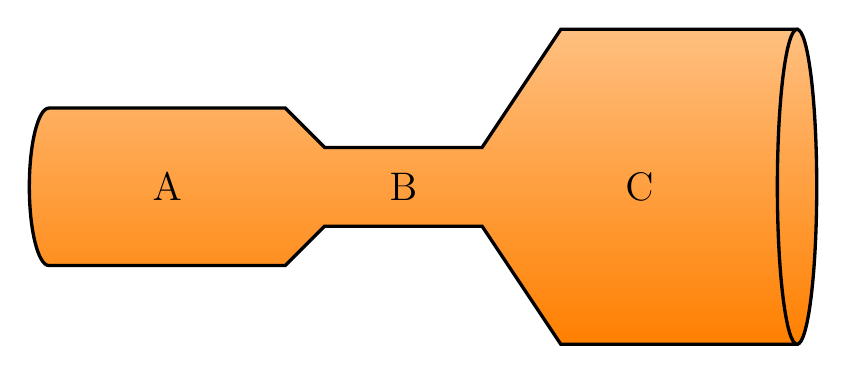
\begin{tikzpicture}
			\draw[very thick, bottom color=orange, top color=orange!50]
				(0,0) -- ++(0,2) -- ++(-3,0) -- ++(-1,-1.5) -- ++(-2,0) -- ++(-.5,.5) -- ++(-3,0)
				arc(90:270:.25cm and 1cm)
				-- ++(3,0) -- ++(.5,.5) -- ++(2,0) -- ++(1,-1.5) -- ++(3,0) -- cycle;
			\draw[very thick, bottom color=orange, top color=orange!50]
				(0,0) circle (.25cm and 2cm);
			\node[font=\Large] at (-8,0) {A};
			\node[font=\Large] at (-5,0) {B};
			\node[font=\Large] at (-2,0) {C};
		\end{tikzpicture}
	\end{center}

	Rank order (from greatest to smallest including ties) the:
	\begin{itemize}
		\item Magnitude of $\ef$ \onslide<2>{\alert{$B>A>C$}}
		\item Conductivity \onslide<2>{\alert{$A=B=C$}}
		\item Current \onslide<2>{\alert{$A=B=C$}}
		\item Current density \onslide<2>{\alert{$B>A>C$}}
	\end{itemize}
	in the labeled regions.
\end{frame}

\begin{frame}{\qnum}
	Inside this resistor setup, what can you conclude about the current density $\vcd$ near the side walls (in steady state)?
	\begin{center}
		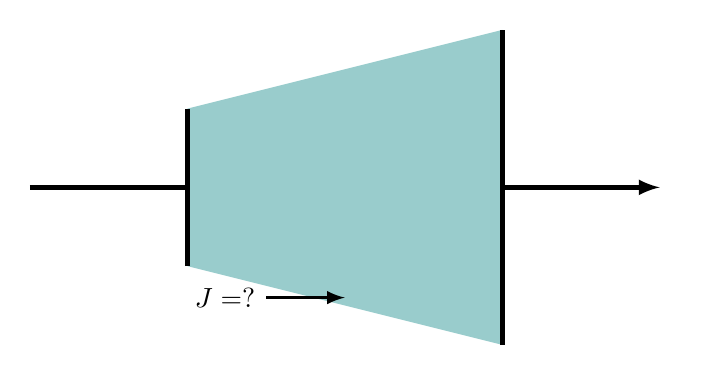
\begin{tikzpicture}
			\draw[ultra thick, -latex] (-4,0) -- (4,0) node[right] {$\mcur$};
			\fill[teal!40] (-2,1) -- (2,2) -- (2,-2) -- (-2,-1);
			\draw[ultra thick] (-2,-1) -- (-2,1) (2,-2) -- (2,2);
			\draw[latex-,very thick] (0,-1.4) -- +(-1,0) node[left] {$J=?$};
		\end{tikzpicture}
	\end{center}
	\begin{enumerate}
		\item \alert<2>{Must be parallel to wall}
		\item Must be perpendicular to wall
		\item Could have both parallel and perpendicular components
		\item There is no way to tell
	\end{enumerate}
\end{frame}

\begin{frame}{\qnum}
	Let's return to our piece of machined copper, looking specifically at the part where it narrows. Assuming there is a steady current flowing through the copper what can you say about $\div\ef$?
	\begin{center}
		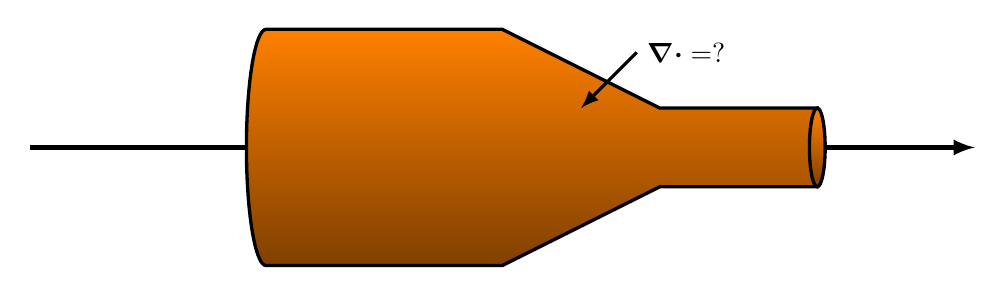
\begin{tikzpicture}
			\draw[ultra thick, -latex] (-6,0) -- (6,0);
			\draw[very thick, bottom color=orange!50!black, top color=orange]
				(4,0) -- ++(0,.5) -- ++(-2,0) -- ++(-2,1) -- ++(-3,0) arc(90:270:.25cm and 1.5cm)
				-- ++(3,0) -- ++(2,1) -- ++(2,0) -- cycle;
			\draw[very thick, bottom color=orange!50!black, top color=orange]
				(4,0) circle (.1cm and .5cm);
			\draw[latex-,very thick] (1,.5) -- +(45:1) node[right] {$\div\ef=?$};
		\end{tikzpicture}
	\end{center}
	\begin{enumerate}
		\item \alert<2>{$\div\ef = 0$}
		\item $\div\ef > 0$
		\item $\div\ef < 0$
		\item It depends on how quickly the copper narrows
	\end{enumerate}
\end{frame}

%\begin{frame}{\qnum}
	%Still looking at the narrowing piece of our copper here. Assuming there is a steady current flowing through the copper what can you say about surface charge collecting on the sloped walls??
	%\begin{center}
		%\begin{tikzpicture}
			%\draw[ultra thick, -latex] (-6,0) -- (6,0);
			%\draw[very thick, bottom color=orange!50!black, top color=orange]
				%(4,0) -- ++(0,.5) -- ++(-2,0) -- ++(-2,1) -- ++(-3,0) arc(90:270:.25cm and 1.5cm)
				%-- ++(3,0) -- ++(2,1) -- ++(2,0) -- cycle;
			%\draw[very thick, bottom color=orange!50!black, top color=orange]
				%(4,0) circle (.1cm and .5cm);
			%\draw[latex-,very thick] (1,.5) -- +(45:1) node[right] {$\div\ef=?$};
		%\end{tikzpicture}
	%\end{center}
	%\begin{enumerate}
		%\item No charge will accumulate
		%\item Positive charge will accumulate
		%\item Negative charge will accumulate
		%\item Positive will accumulate on the top and negative on the bottom
	%\end{enumerate}
%\end{frame}








\end{document}
